\documentclass[fontsize=8pt, a4paper, landscape, fleqn]{scrartcl}

\usepackage[utf8]{inputenc}
\usepackage[english]{babel}
%\usepackage[standardsections]{scrhack}
%\usepackage[raggedright]{titlesec} %% Gives warnings
\usepackage{xcolor}
\usepackage{enumerate, enumitem, ulem, graphicx, multirow, comment}
\usepackage{listings}
\usepackage{wrapfig} 
\usepackage{titlesec}     % For customizing section titles
%Graph
\usepackage{tikz}
\usetikzlibrary{positioning}
\usetikzlibrary{trees}
\usepackage{pgfplots}

%Page reference
\usepackage{hyperref}
\usepackage{xparse,nameref}
\hypersetup{
pdfborder={0 0 0}, % Add this line to remove the link border
}

%code layout
\definecolor{sec}{RGB}{40,56,71}
\definecolor{subsec}{RGB}{72,98,124}
\definecolor{subsubsec}{RGB}{102,141,178}
\definecolor{codegreen}{rgb}{0,0.6,0}
\definecolor{codegray}{rgb}{0.5,0.5,0.5}
\definecolor{codepurple}{rgb}{0.58,0,0.82}
\definecolor{backcolour}{RGB}{240,240,240}
\usepackage{tcolorbox}
\tcbuselibrary{minted, breakable}

% Define custom colors
\definecolor{sectioncolor}{RGB}{64, 64, 64}       % Dark Gray
\definecolor{subsectioncolor}{RGB}{70, 130, 180}  % Steel Blue

% Custom section and subsection commands with unified styling
\renewcommand{\section}[1]{%
    \noindent\colorbox{sectioncolor}{%
        \parbox{\dimexpr\columnwidth-2\fboxsep}{\color{white}\textbf{#1}}}%
    \vspace{0.5mm}% Optional spacing after the section
}

\renewcommand{\subsection}[1]{%
    \noindent\colorbox{subsectioncolor}{%
        \parbox{\dimexpr\columnwidth-2\fboxsep}{\color{white}\textbf{#1}}}%
    \vspace{0.5mm}% Optional spacing after the subsection
}

% Optional: Customize subsubsection or other title levels
\renewcommand{\subsubsection}[1]{%
    \noindent\textbf{\textit{\color{subsectioncolor}#1}}% Italic with subsection color
    \vspace{1mm}% Optional spacing after subsubsection
}
%Layout
\usepackage{multicol, geometry, titlesec, xcolor}
\geometry{margin=0.2cm}
%\titlespacing{\section}{0pt}{3pt}{1pt}
%\titlespacing{\subsection}{0pt}{3pt}{1pt}
%\titlespacing{\subsubsection}{0pt}{3pt}{1pt}
\parindent 0pt

%Remove numbering
\pagestyle{empty} 
%\pagenumbering{arabic}

\setlist[itemize]{leftmargin=2mm, itemsep=0mm} %{nosep}
\setlist[enumerate]{leftmargin=3mm, nosep} %{nosep}

\newlength{\breite}
\setlength{\breite}{0.5pt}
\setlength{\columnseprule}{\breite}

\usepackage{graphicx}

%Style code
\usepackage{minted}
\lstdefinestyle{mystyle}{
    backgroundcolor=\color{backcolour},
    commentstyle=\color{codegreen},
    keywordstyle=\color{blue},
    numberstyle=\tiny\color{codegray},
    stringstyle=\color{codepurple},
    basicstyle=\ttfamily,
    breakatwhitespace=false,
    breaklines=true,
    captionpos=b,
    keepspaces=true,
%    numbers=left,
    numbersep=5pt,
    showspaces=false,
    showstringspaces=false,
    showtabs=false,
    tabsize=2,
}
\lstset{style=mystyle}

%Mathematics
\usepackage{amsmath, amstext, amssymb, mathtools, esint, polynom}
\allowdisplaybreaks 

%Document file
\begin{document}
\begin{multicols*}{3}[\raggedcolumns]


\section{Atmospheric General Circulation}
\noindent\textcolor{orange}{
Goal: Understand the structure, drivers, and variability of the general circulation of the atmosphere, and how it connects to weather, climate, and climate change.\\
Flow: Starts with observed circulation features, proceeds to explain the underlying physics (energy balance, rotation, instability), highlights the role of eddies, and ends with climate change responses.
}

\subsection{Observed Features of the General Circulation}
\begin{itemize}
    \item \textbf{Definition:} The general circulation is the full statistical description of large-scale atmospheric motions.
    \item \textbf{Surface winds:} 
    \begin{itemize}
        \item Persistent easterly trade winds in the tropics, especially between 10–30° latitude.
        \item Westerly winds dominate in midlatitudes.
    \end{itemize}
    \item \textbf{Precipitation patterns:}
    \begin{itemize}
        \item ITCZ and SPCZ are zones of intense precipitation and low-level convergence.
        \item Dry subtropics arise from subsiding branches of circulation cells.
        \item \textbf{P–E}: Positive (wet) where air ascends and moisture converges; negative (dry) where it descends.
    \end{itemize}
    \item \textbf{Jet streams:} 
    \begin{itemize}
        \item Subtropical and midlatitude jets are upper-level westerlies intensified at steep meridional temperature gradients.
    \end{itemize}
    \item \textbf{Temperature structure:} 
    \begin{itemize}
        \item Tropics show weak meridional gradients; strong gradients exist in midlatitudes.
        \item These gradients define the location and strength of jet streams.
    \end{itemize}
    \item \textbf{Surface temperatures:}
    \begin{itemize}
        \item The circulation acts to reduce the equator-to-pole temperature gradient.
    \end{itemize}
    \item \textbf{Cloud cover:}
    \begin{itemize}
        \item Thick clouds in convergence/ascent regions; shallow clouds in descent zones.
    \end{itemize}
\end{itemize}

\subsection{Why Is There a General Circulation?}
\begin{itemize}
    \item \textbf{Energy imbalance:} Net radiative input at low latitudes exceeds output, necessitating poleward energy transport.
    \item \textbf{Earth's rotation:} As air moves poleward, conservation of angular momentum leads to zonal acceleration—producing westerlies.
    \item \textbf{Angular momentum paradox:}
    \begin{itemize}
        \item Simple Hadley theory overpredicts wind speeds aloft.
        \item Real atmosphere departs from angular momentum conservation due to eddy momentum fluxes.
    \end{itemize}
\end{itemize}

\subsection{Zonal Circulation and Meridional Energy Transport}
\begin{itemize}
    \item \textbf{Hadley Cell:} Equator-to-30° overturning, thermally direct, with strong upper-level zonal winds.
    \item \textbf{Ferrel Cell:} Midlatitude indirect cell, maintained by eddy heat and momentum fluxes.
    \item \textbf{Polar Cell:} Weak thermally direct circulation at high latitudes.
    \item \textbf{Meridional heat transport:} Atmosphere and ocean together move energy poleward, with peak atmospheric transport near 40°.
\end{itemize}

\subsection{Baroclinic Instability and the Role of Eddies}
\begin{itemize}
    \item \textbf{Instability onset:} Strong jets become baroclinically unstable, generating eddies (e.g., extratropical cyclones).
    \item \textbf{Eddy effects:}
    \begin{itemize}
        \item Transport heat poleward (eddy heat flux divergence drives vertical motion in Ferrel cell).
        \item Transport momentum equatorward and downward (sustains surface westerlies, modifies jets).
    \end{itemize}
    \item \textbf{Jet distinction:}
    \begin{itemize}
        \item \textit{Subtropical jet:} From angular momentum conservation at Hadley cell edge.
        \item \textit{Eddy-driven jet:} Maintained by eddy momentum convergence in midlatitudes.
    \end{itemize}
\end{itemize}

\subsection{Eddies as Weather Systems}
\begin{itemize}
    \item \textbf{Rossby waves:} Baroclinic eddies propagate along jets and break, transferring energy and momentum.
    \item \textbf{Momentum budget:}
    \begin{itemize}
        \item Midlatitude eddies converge momentum, sustaining surface westerlies.
        \item In the subtropics, they extract momentum, weakening subtropical jets.
    \end{itemize}
    \item \textbf{Heat budget:}
    \begin{itemize}
        \item Ferrel cell motion driven by eddy heat flux divergence/convergence, analogous to Hadley cell's latent/radiative balance.
    \end{itemize}
\end{itemize}

\subsection{Climate Change Impacts on the Circulation}
\begin{itemize}
    \item \textbf{Polar amplification:} Weakens meridional temperature gradient—suggesting weaker jets.
    \item \textbf{Tropical amplification:} Moisture increase enhances upper-tropospheric warming—suggesting stronger jets.
    \item \textbf{Poleward shifts:} Jets, storm tracks, and Hadley cell edges shift poleward.
    \item \textbf{Uncertainty:} Competing mechanisms (moisture vs. gradient reduction) create uncertainty in net response.
\end{itemize}

\subsection{Key Insights}
\begin{itemize}
    \item General circulation shapes winds, precipitation, and clouds globally and seasonally.
    \item Driven by energy imbalances and shaped by rotation and instabilities.
    \item Eddies are essential to midlatitude dynamics, enabling heat and momentum redistribution.
    \item Climate change modifies circulation through altered heating patterns and humidity feedbacks.
\end{itemize}









\section{The ocean: General circulation and climate}
\noindent\textcolor{orange}{
Goal: Understand the role of the ocean in Earth's climate system, its physical structure and circulation, and its response to anthropogenic forcing.\\
Flow: From ocean heat content and geometry to salinity, density, overturning, tracer evidence, and biogeochemical coupling.
}

\subsection{Central role in the climate system}
\begin{itemize}
    \item Oceans store $>$90\% of excess heat from global warming.
    \item Major regulator of the water and carbon cycles.
    \item Influences both abrupt and gradual climate variability.
\end{itemize}

\subsection{Physical setting}
\begin{itemize}
    \item Covers $\sim$71\% of Earth's surface.
    \item Southern Ocean connects major ocean basins and enables global exchange.
    \item Vast majority of Earth’s water is saline; only 2.5\% is freshwater.
\end{itemize}

\subsection{Key physical properties of seawater}

\begin{figure}[H]
    \centering
    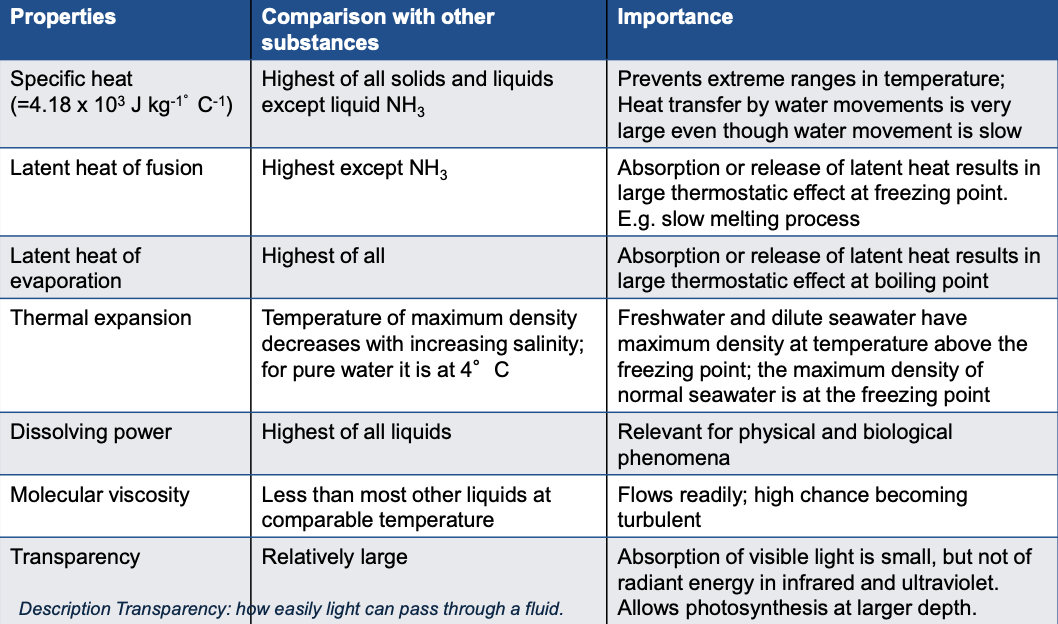
\includegraphics[width=0.9\linewidth]{CS/img/saltwater_table.png}
\end{figure}


\begin{itemize}
    \item High specific and latent heat capacities $\Rightarrow$ large thermal inertia.
    \item Density varies with temperature, salinity, pressure:
    \[
    \rho(T,S) \approx \rho_0(1 - \alpha_T(T - T_0) + \beta_S(S - S_0))
    \]
    \item Typical ranges: $T = -2^\circ C$ to $30^\circ C$, $S \approx 34$–$36$ PSU.
\end{itemize}

\subsection{Stratification and vertical structure}
\begin{itemize}
    \item Surface mixed layer, thermocline, and abyssal layer.
    \item Sharp vertical gradients define water masses and affect mixing.
\end{itemize}

\subsection{Ocean circulation}
\begin{itemize}
    \item \textbf{Wind-driven (upper ocean):} Includes Ekman transport, geostrophic currents, gyres, boundary currents (e.g., Gulf Stream).
    \item \textbf{Density-driven (deep ocean):} Thermohaline circulation forms overturning cells based on $T$–$S$ contrasts.
    \item Southern Ocean plays a central role in global upwelling and mixing.
\end{itemize}


\begin{figure}[H]
    \centering
    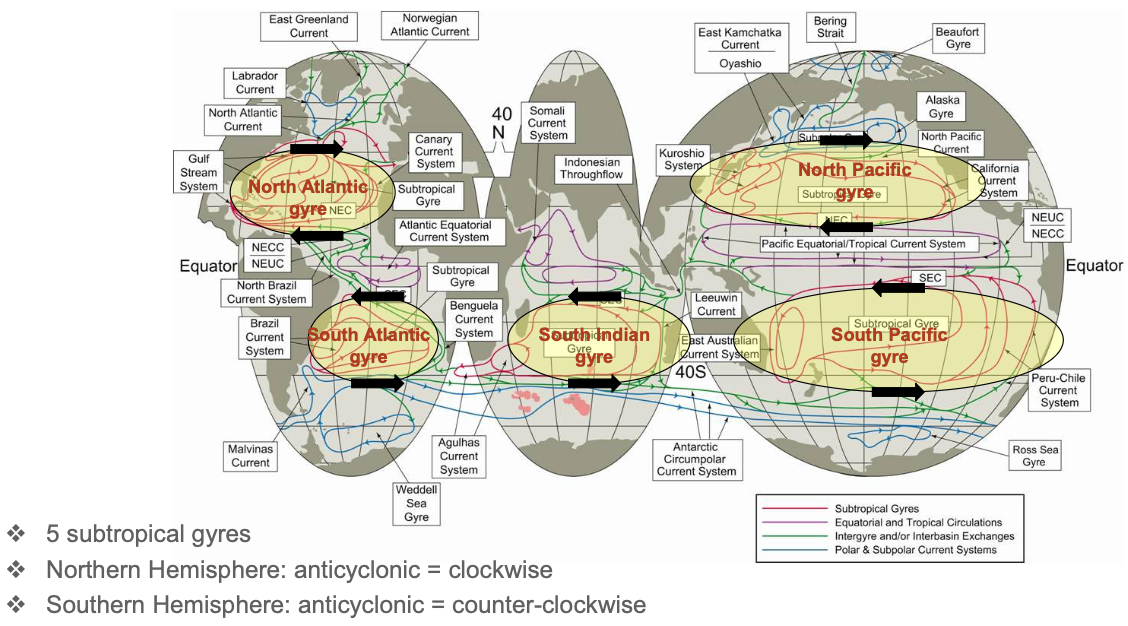
\includegraphics[width=0.9\linewidth]{CS/img/Subtropical_Gyres.png}
    \caption{Subtropical Gyres: Anticyclonic Circulations}
\end{figure}


\begin{figure}[H]
    \centering
    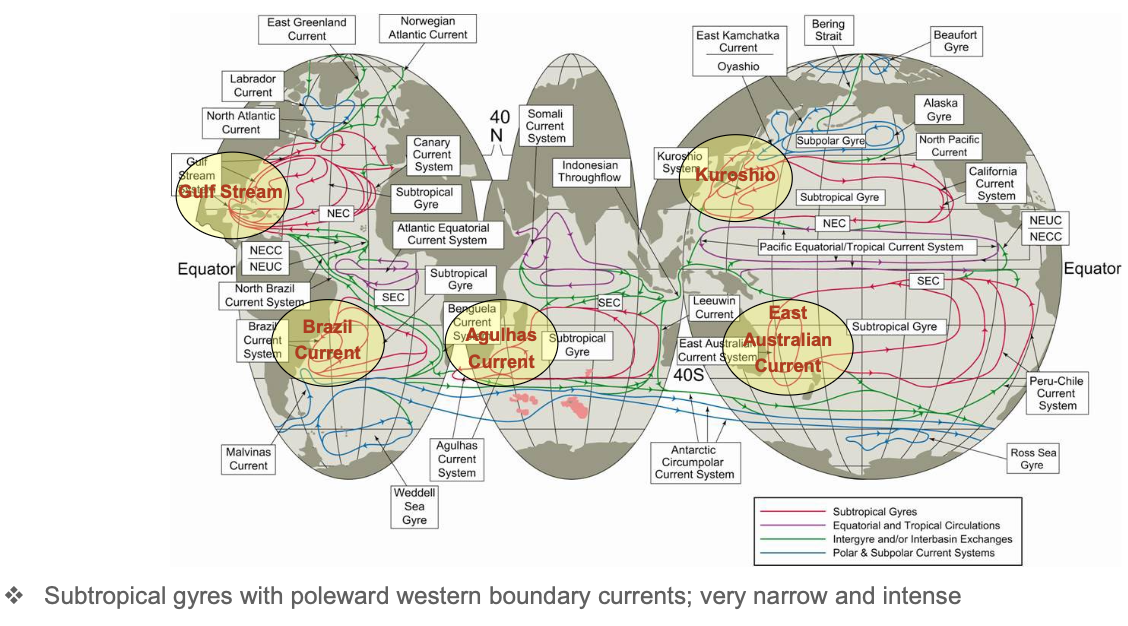
\includegraphics[width=0.9\linewidth]{CS//img/western_bound.png}
    \caption{Subtropical Gyres: Western Boundary Current}
\end{figure}

\begin{figure}[H]
    \centering
    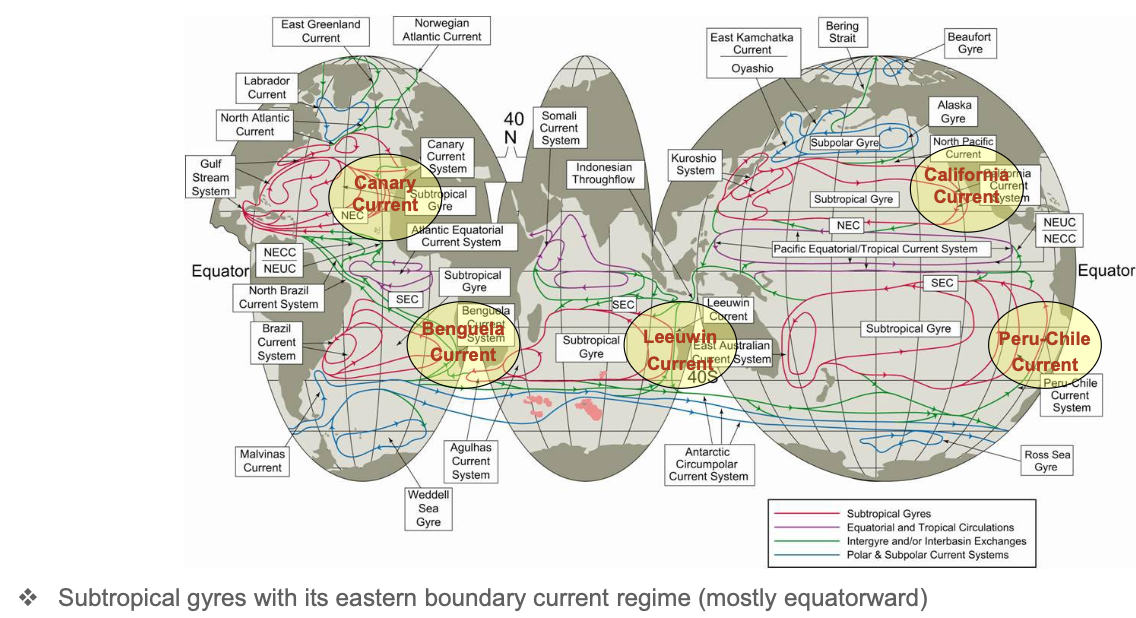
\includegraphics[width=0.9\linewidth]{CS//img/eastern_bound.png}
    \caption{Subtropical Gyres: Eastern Boundary Current}
\end{figure}

\begin{figure}[H]
    \centering
    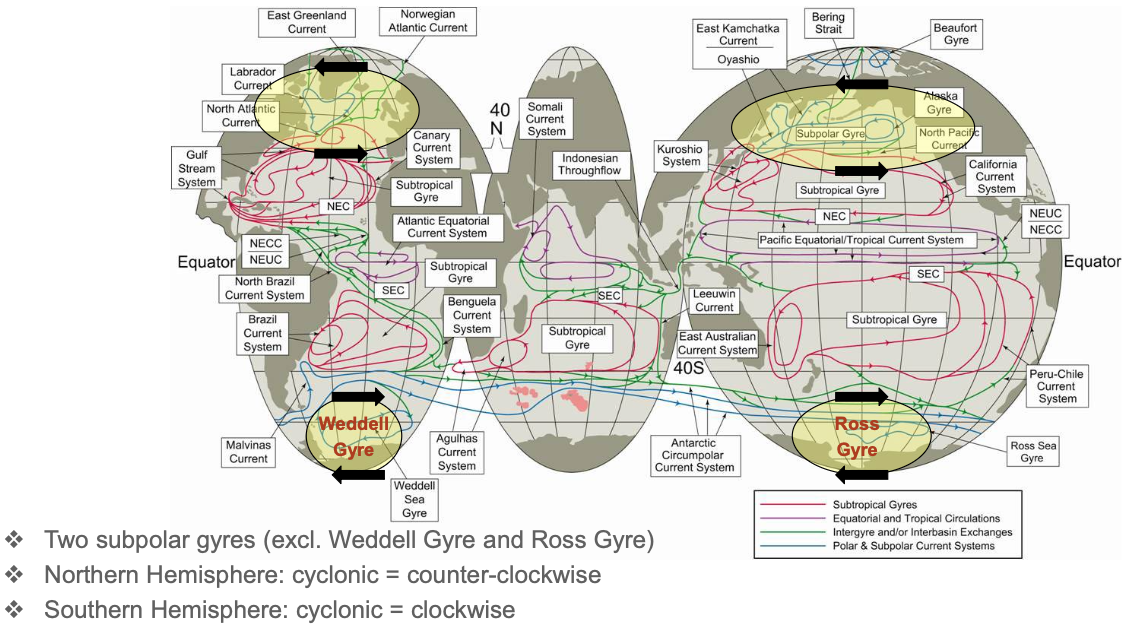
\includegraphics[width=1\linewidth]{CS//img/cyclonic_circulations.png}
    \caption{Subpolar Gyres: Cyclonic Circulations}
\end{figure}

\begin{figure}[H]
    \centering
    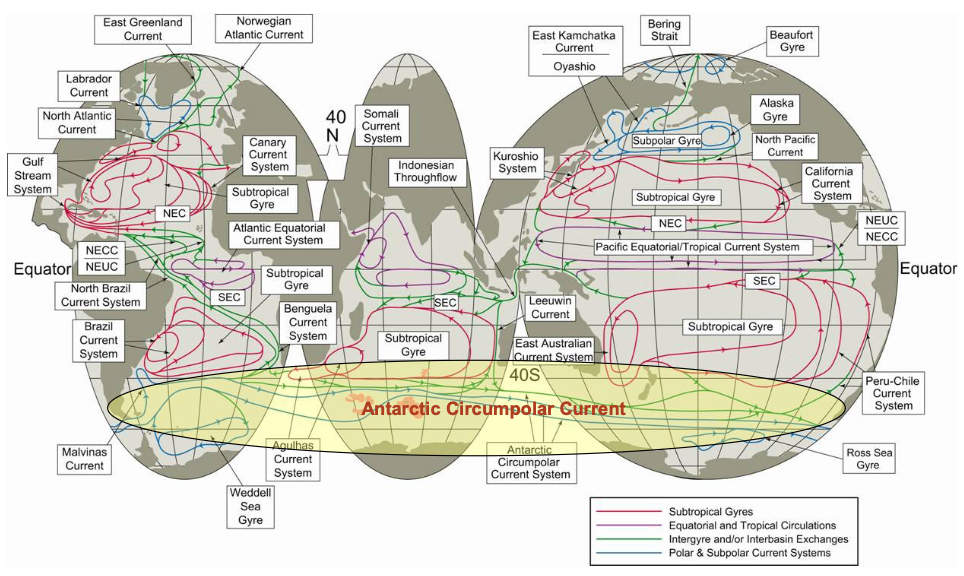
\includegraphics[width=0.9\linewidth]{CS//img/circumpolar_current.png}
    \caption{Antarctic Circumpolar Current}
\end{figure}

\subsection{Schematic of Wind Patterns}

\begin{figure}[H]
    \centering
    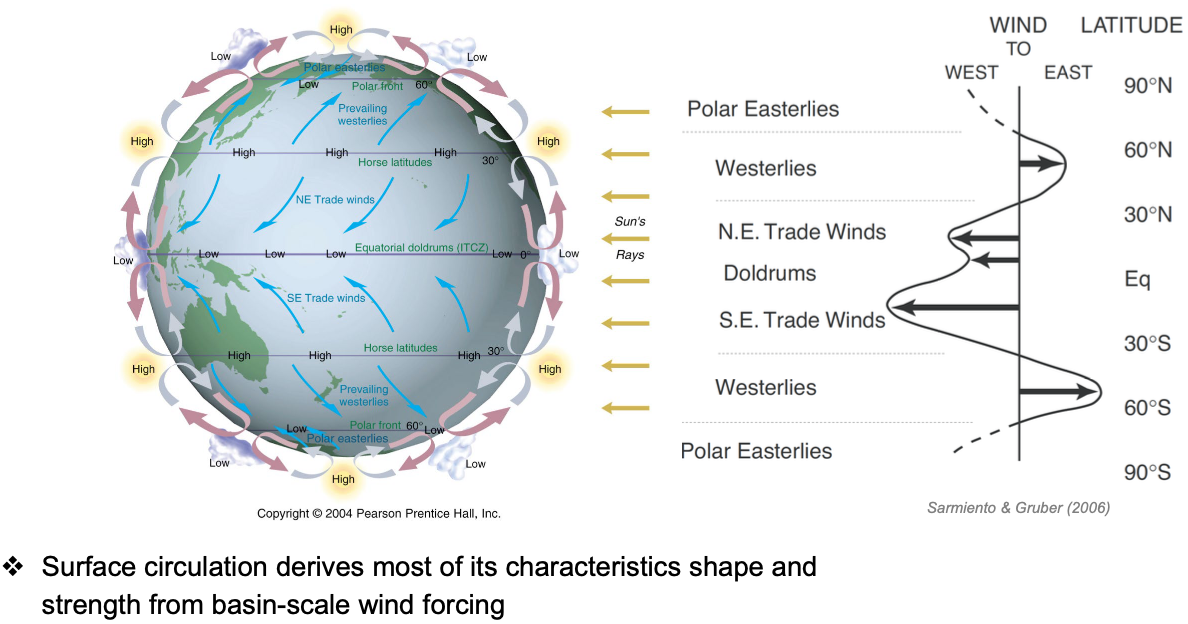
\includegraphics[width=0.7\linewidth]{CS//img/Schematic_Wind.png}
\end{figure}

\subsection{Water masses and tracers}
\begin{itemize}
    \item Identified by $T$–$S$ signatures and chemical tracers (CFCs, $\Delta^{14}$C, oxygen).
    \item NADW, AABW, AAIW, etc., represent distinct sources and sinks.
    \item Tracers like CFCs and $\Delta^{14}$C allow dating and tracking ventilation.
\end{itemize}

\subsection{Global overturning circulation}
\begin{itemize}
    \item Driven by sinking in the North Atlantic and upwelling in the Southern Ocean.
    \item Modulates heat transport, climate variability, and carbon uptake.
    \item Collapse scenarios (e.g., AMOC shutdown) have major climate implications.
\end{itemize}

\subsection{Biogeochemical cycling}
\begin{itemize}
    \item Ocean physics and biology regulate the biological pump.
    \item Upwelling sustains high productivity regions.
    \item Key organisms: diatoms, coccolithophores, cyanobacteria.
\end{itemize}

\subsection{Climate implications}
\begin{itemize}
    \item Ocean warming, acidification, and sea level rise.
    \item Major role in buffering anthropogenic CO$_2$ (195 ± 40 GtC since 1750).
    \item Variability (ENSO, decadal) and long-term trends affect Earth’s climate feedbacks.
\end{itemize}

\section{Weather Systems, Clouds, and Aerosols in the Climate System}
\noindent\textcolor{orange}{
Goal: Understand how specific weather systems contribute to climate risks, and how clouds and aerosols modulate those risks in the climate system.\\
Flow: From weather system typology and case studies to cloud processes, aerosol interactions, and geoengineering risks.
}

\subsection{Weather Systems and Climate Risks}
\begin{itemize}
    \item \textbf{Types of systems:} Cyclones (lows), blocking highs, convection, Föhn, fronts.
    \item \textbf{Impacts:} Drive most extreme events — floods, storms, heatwaves, droughts.
    \item \textbf{Key features:}
    \begin{itemize}
        \item \textbf{Cyclones:} Storms, intense precipitation.
        \item \textbf{Blocking highs:} Long-lasting anomalies (e.g., heatwaves, cold spells).
        \item \textbf{Föhn:} Orographic winds with temperature and humidity gradients.
    \end{itemize}
    \item \textbf{Predictability:} Limited due to high variability and chaotic dynamics.
\end{itemize}

\subsection{Case Studies of Extreme Events}
\begin{itemize}
    \item \textbf{Arctic Warming Event (Dec 2015):}
    \begin{itemize}
        \item +8.7°C in Svalbard — higher than summer mean.
        \item Driven by warm air transport: near-surface from Sahara, aloft from Canada with adiabatic descent.
        \item Enabled by strong W-E pressure gradient and polar-ward jet.
    \end{itemize}

    \item \textbf{European Flood (June 2013):}
    \begin{itemize}
        \item Cyclonic storm track enabled persistent precipitation.
        \item Dominated by \textbf{Warm Conveyor Belts (WCBs)}:
        \begin{itemize}
            \item Rapidly ascending, moisture-laden airflows moving poleward.
            \item Drive significant winter precipitation in Europe.
        \end{itemize}
    \end{itemize}

    \item \textbf{Pacific Northwest Heatwave (June 2021):}
    \begin{itemize}
        \item Caused by a blocking anticyclone and adiabatic warming from descending air.
        \item Amplified by clear-sky radiative heating and warm air advection.
    \end{itemize}
\end{itemize}

\subsection{WCBs and Blocking Climatology}
\begin{itemize}
    \item \textbf{WCBs:} Frequent in midlatitudes; major precipitation drivers.
    \item \textbf{Blocking:} Long-lived, quasi-stationary high-pressure systems.
    \begin{itemize}
        \item Block the westerlies, shift storm tracks.
        \item Occur preferentially in winter (e.g., over NE Atlantic, Siberia).
        \item Can cause prolonged heat/cold events.
    \end{itemize}
\end{itemize}

\subsection{Weather Prediction as an Initial Value Problem}
\begin{itemize}
    \item Governed by known physical laws (momentum, thermodynamics, radiation).
    \item Solved numerically via data assimilation + ensemble prediction.
    \item \textbf{Chaos:} Small differences in initial conditions grow rapidly.
    \item Predictability horizon: hours (convective events) to weeks (blocking).
\end{itemize}

\subsection{Cloud Processes and Radiative Balance}
\begin{itemize}
    \item \textbf{Cloud formation requires:} Moisture, vertical lifting, aerosols (as CCN).
    \item \textbf{Formation mechanisms:} Frontal zones, orographic lifting, surface heating.
    \item \textbf{Radiative effects:}
    \begin{itemize}
        \item \textbf{Low clouds:} Reflect sunlight $\rightarrow$ cooling.
        \item \textbf{High clouds:} Trap outgoing IR $\rightarrow$ warming.
    \end{itemize}
    \item Net effect depends on cloud type, height, thickness, and coverage.
\end{itemize}

\subsection{Aerosols and Their Climate Effects}
\begin{itemize}
    \item \textbf{Sources:} Natural (dust, sea salt, biogenic), anthropogenic (soot, sulfates).
    \item \textbf{Size modes:} Nucleation (nm), accumulation ($\sim$0.1–1$\mu$m), coarse ($>$1$\mu$m).
    \item \textbf{Effects:}
    \begin{itemize}
        \item \textbf{Direct:} Scatter and absorb solar radiation.
        \item \textbf{Indirect:} Act as CCN $\rightarrow$ smaller droplets, brighter clouds, suppressed precipitation.
    \end{itemize}
    \item \textbf{Historical impact:} Mid-20th-century aerosol emissions led to global dimming; recent reduction $\rightarrow$ rebrightening.
\end{itemize}

\subsection{Climate Engineering via Aerosols and Clouds}
\begin{itemize}
    \item \textbf{SRM methods:}
    \begin{itemize}
        \item Stratospheric aerosol injection (e.g., sulfate layer like Mt. Pinatubo).
        \item Marine cloud brightening (more low clouds over oceans).
        \item Cirrus thinning (increases outgoing longwave radiation).
    \end{itemize}
    \item \textbf{Limitations and risks:}
    \begin{itemize}
        \item Regional climate disruption, termination shock, limited effect on ocean acidification.
        \item Ethical and governance concerns.
    \end{itemize}
    \item \textbf{Cloud seeding experiments:} Ongoing (e.g., in Eriswil, Switzerland), targeting supercooled liquid clouds.
\end{itemize}

\subsection{Key Takeaways}
\begin{itemize}
    \item Weather systems drive short-term extremes and interact with climate trends.
    \item Cloud–aerosol interactions significantly impact Earth's energy budget and remain uncertain.
    \item Predictability is fundamentally limited but can be improved via better observations and ensemble techniques.
    \item Climate engineering may reduce warming temporarily but carries severe risks and cannot replace emission reductions.
\end{itemize}

\section{Climate and weather risks }

\end{multicols*}
\end{document}